%% This is file `prletters-template.tex',
%% 
%% Copyright 2013 Elsevier Ltd
%% 
%% This file is part of the 'Elsarticle Bundle'.
%% ---------------------------------------------
%% 
%% It may be distributed under the conditions of the LaTeX Project Public
%% License, either version 1.2 of this license or (at your option) any
%% later version.  The latest version of this license is in
%%    http://www.latex-project.org/lppl.txt
%% and version 1.2 or later is part of all distributions of LaTeX
%% version 1999/12/01 or later.
%% 
%% The list of all files belonging to the 'Elsarticle Bundle' is
%% given in the file `manifest.txt'.
%% 
%% Template article for Elsevier's document class `elsarticle'
%% with harvard style bibliographic references
%%
%% $Id: prletters-template-with-authorship.tex 69 2013-07-15 10:15:25Z rishi $
%%
%% This template has no review option
%% 
%% Use the options `twocolumn,final' to obtain the final layout
\documentclass[times,twocolumn,final,authoryear]{elsarticle}

%% Stylefile to load PR Letters template
\usepackage{prletters}
\usepackage{framed,multirow}

%% The amssymb package provides various useful mathematical symbols
\usepackage{amssymb}
\usepackage{latexsym}

% Following three lines are needed for this document.
% If you are not loading colors or url, then these are
% not required.
\usepackage{url}
\usepackage{xcolor}
\definecolor{newcolor}{rgb}{.8,.349,.1}

%%%%%%%%%%%%%%%
% jdelatorre added header
\usepackage{tikz}
\usepackage{blindtext, graphicx}
\usepackage{smartdiagram}
\newcommand{\degree}{\ensuremath{^{\circ}}\xspace} % adds degree sign 
\usepackage[utf8]{inputenc}
\usepackage[T1]{fontenc} % adds capability to < sign
\usepackage{mathptmx}
\usepackage{amsmath}

% forced line break inside a tabular cell
\newcommand{\specialcell}[2][c]{%
	\begin{tabular}[#1]{@{}c@{}}#2\end{tabular}}

% use it for example as \specialcell[t]{Foo\\bar} or \specialcell{Foo\\bar}
%%%%%%%%%%%%%%%

\journal{Pattern Recognition Letters}

\begin{document}

\thispagestyle{empty}
                                                             
\clearpage


\ifpreprint
  \setcounter{page}{1}
\else
  \setcounter{page}{1}
\fi

\begin{frontmatter}

\title{Weighted kappa loss function for multi-class classification of ordinal data in deep learning}

\author[1]{Jordi \snm{de la Torre}} 
\author[1]{Domenec \snm{Puig}}
\author[1]{Aida \snm{Valls}\corref{cor1}}

\cortext[cor1]{Corresponding author: 
	Tel.: +34-977-559-688;  
	fax: +34-977-559-710;}
\ead{aida.valls@urv.cat}

\address[1]{Departament d'Enginyeria Inform\`{a}tica i Matem\`{a}tiques\\ Universitat Rovira i Virgili \\ Avinguda Pa\"{i}sos Catalans, 26 \\ ES-43007 Tarragona}

\received{30 Jan 2017}
\finalform{30 Jan 2017}
\accepted{30 Jan 2017}
\availableonline{30 Jan 2017}
\communicated{S. Sarkar}


\begin{abstract}

Weighted Kappa is a index of reference used in many diagnosis systems to compare the agreement between different raters. This index can be also used to evaluate the performance of automatic classification methods against the gold standard given by an expert (or from a consensus of an expert group). On the other hand, in the last years, deep learning has achieved a great importance as a new machine learning method. The usual loss function used in deep learning for multi-class classification is the logarithmic loss. In this paper we explore the direct use of a weighted kappa loss function for multi-class classification of ordinal data, also known as ordinal regression. Three classification problems are solved in the paper using these two loss functions. Results confirm that better classification is made when the model is constructed with the optimization of kappa instead of logarithmic loss.

\end{abstract}

\begin{keyword}
\MSC 62H35\sep 82C32\sep 62M45
\KWD deep learning\sep convolutional neural networks\sep supervised learning\sep computer vision\sep diabetic retinopathy\sep weighted kappa

%\sep ordinal regression \sep cohen's kappa\sep loss function\sep ordinal data
%% MSC codes here, in the form: \MSC code \sep code
%% or \MSC[2008] code \sep code (2000 is the default)
\end{keyword}

\end{frontmatter}

%\linenumbers

\section{Introduction}

Deep Learning is a set of Machine Learning techniques 
for automatically constructing a model with multiple levels of representation from the underlying distribution of a large set of examples, with the final objective of mapping a high-multidimensional input into a smaller multidimensional output (f: $\mathbb{R}^{n} 
\mapsto \mathbb{R}^{m}, n \gg m$). 
This mapping allows the classification of multidimensional objects into a small number of categories. The model is composed by many neurons that are organized in layers and blocks of layers, using a cascade of layers in a hierarchical way. Every neuron receives the input from a predefined set of neurons. Every connection has a parameter that corresponds to the weight of the connection. 
The function of every neuron is to make a transformation of the received inputs into a calculated output value. For every incoming connection, the weight is multiplied by the input value received by the neuron and the aggregated value that used by an activation function that calculates the output of the neuron. The parameters are usually optimized using a stochastic gradient descent algorithm that minimizes a predefined loss function. The parameters of the network are updated after backpropagating the loss function gradients through the network. These hierarchical models are able to learn multiple levels of representation that correspond to different levels of abstraction, which enables the representation of complex concepts in a compressed way \citep{nature-deep-learning}, \citep{888}, \citep{Bengio:2013:RLR:2498740.2498889}, \citep{bengio-2009}.

Deep Learning methods have been used extensively in the last years for many automatic classification tasks. For the case of image analysis, the usual procedure consists on extracting the important features with a set of convolutional layers and, after that, make a final classification with these features using a set of fully connected layers. Finally, a soft-max output layer gives as a result the predicted output probabilities of the set of classes predefined in the model. During training the model parameters are changed using a gradient-based optimization algorithm, which minimizes a predefined loss function. For multi-class classification the standardized loss function to use is the logarithmic loss \citep{Goodfellow-et-al-2016}.

Once the classifier has been trained (i.e. the parameters of the different layers of the model have been fixed), the quality of the classification outputs predicted by the model are compared against the correct "`true"' values stored on a labeled dataset. This data is considered as the gold standard, coming from the consensus of the knowledge of a human experts group.

Several quality measures exist in the literature of machine learning and statistics \citep{mehdiyev2016evaluating}. 
Kappa index is well-known statistic coefficient defined by Cohen \citep{cohen1960coefficient} to measure inter-rater agreement on classifying elements into a set of categories (i.e. disjoint classes).
Later, Weighted Kappa index was defined for the case of ordered categories (i.e. from best to worst). In this coefficient disagreements are treated differently than in the original Cohen's Kappa \citep{cohen1968weighted}. 

Weighted Kappa index ($\kappa$) is used in many medical diagnosis systems because the diseases have different degrees of severity, which are naturally ordered from mild to the most critical cases. If the diagnose is based on image analysis, the classification is even more difficult because in the interpretation of the image data normally is present some level of subjectivity that sometimes makes the conclusions of different experts to differ \citep{hripcsak2002measuring}.
Weighted kappa is able to measure the level of discrepancy of a set of diagnosis made by different raters over the same population \citep{viera2005understanding}. Depending on the value of the index, the strength of agreement between the raters can be evaluated (see table \ref{tab:kappa_int}). 

Examples of the usage of the $\kappa$ index for measuring inter-rater agreement in the medical context are: the measure of reliability in ultrasound scans interpretation \citep{hintz2007interobserver}, the evaluation of expert agreement in diagnosis of glaucoma \citep{varma1992expert}, the evaluation of reliability of radiographic assessment \citep{gunther1999reliability}, the inter-observer agreement evaluation in diabetic retinopathy detection \citep{patra2009interobserver}, among many others. 

$\kappa$ takes into account the ordering of the classes and penalizes the erroneous predictions in function of the distance between the real and the predicted class. In that way, a failure in a prediction that is close to the real category is considered better than a prediction that is farther. The penalization weights depend on the type of the chosen weighted kappa. In a linear penalization the weight is proportional to the distance, in the quadratic weighted kappa ($\kappa$) - the one studied in this paper - the penalization is proportional to the square of the distance. %Weighted kappa allow the definition of weight matrices of all kinds. 


\begin{table}
	\caption{\label{tab:kappa_int}Table for interpretation of Weighted Kappa, after Landis \& Koch (1977)}	
	\centering
	\begin{tabular}{llr}
		\hline
		$\kappa$    & Strength of agreement \\
		\hline
		<0.20 		& Poor \\
		0.21-0.40 	& Fair \\
		0.41-0.60 	& Moderate \\
		0.61-0.80 	& Good \\
		0.81-1.00 	& Very good \\
		\hline
	\end{tabular}
\end{table}

In this paper, we study the direct optimization of the $\kappa$ index, using it not only as a evaluation function but also as loss function during the training of the model. In the cases where there is some order relation between the output classes, the optimization of the loss function needs to learn this order from the available data to make good predictions. Our hypothesis is that a loss function that encodes such a priori order knowledge can perform better or faster than the usual logarithmic loss function, due to the fact that we are including this additional information known beforehand. 

To prove this hypothesis, we use 3 problems of different complexity and with  different type of data. Moreover, the neural net model required in each case has an increasing complexity.

The last case that we study, the more complex one, is a diabetic retinopathy image classification problem. Diagnosis of diabetic retinopathy from eye fundus images has been previously studied and it is considered a hard problem, because the classification into levels of severity is based on indicators that are difficult to detect in the images \citep{DBLP:conf/ccia/TorreVP16}, \citep{DBLP:conf/ccia/Escorcia-Gutierrez16}. 
We check its stability and compare the performance of the results obtained from the use of the standard logarithmic loss against the results obtained from the optimization of $\kappa$. 

The study is organized as follows: in section 2 we present the deep learning standard method of optimization showing the standardized loss function used for classification, in section 3 we propose the new cost function for multi-class classification of ordinal data (ordinal regression) with all the mathematical equations required for the optimization using first order gradient descent algorithms, in section 4 we define the experiments, in section 5 we present the results obtained and finally in section 6 we present the conclusions of the paper.

\section{Deep learning method}

Supervised deep learning techniques are recently used extensively for many automatic classification tasks. In the case of images, most of the state of the art methods are based on the use of deep convolutional neural networks (DCNN): CIFAR-10 \citep{DBLP:journals/corr/Graham14a}, CIFAR-100 \citep{DBLP:journals/corr/ClevertUH15}, STL10 \citep{DBLP:journals/corr/DundarJC15}, SVHN \citep{DBLP:journals/corr/LiaoC15a}, ImageNet \citep{NIPS2012_4824}, among many others. These techniques are focused on learning multiple levels of representation and abstraction that help to make sense of the hidden information in data such as images. In this way, having a complete set of correctly classified images and without any a priori understanding of the features, the model is able to learn the properties of the image that minimize a defined cost function that is direct or indirectly related with the classification score index to optimize. 

\begin{figure}[!h]
	\centering
	\smartdiagramset{back arrow disabled=true}
	\resizebox{.9\linewidth}{!}{\smartdiagram[flow diagram:horizontal]{Image Input, Feature Extraction Layers, Classification Layers, Class Probability, Cost\\Function}}
	\caption{High level description of a deep learning image classification scheme}
	\label{fig:classification}
\end{figure}


As shown in Fig. \ref{fig:classification} for image classification, several convolutional neural networks are optimized for making  a good feature extraction. These layers are followed by one or more classification layers. Finally, the last output layer is formed by as many outputs as classes to predict. In the output layer is usual to have a soft-max function that represents the output probability of every class to predict. Normally, the class assigned to the image is the one with the highest value of probability. 

The main parameters to define are: total number of layers, the size of the convolutions with its stride and padding, the activation function to use, the number of convolutional filters for every layer and the type and number of elements of classification layer (fully connected or convolutional).

Moreover, once the architecture of the DCNN has been defined, the neural network has a set of parameters to optimize in order to achieve the most accurate prediction of the data. This is done by optimizing a function of the output variables, called \textit{loss function}. This function depends on the output probabilities given by the model and it is defined in a way that minimizing it, maximizes the probability of the correct class. If the defined function is differentiable with respect to the output variables, then is possible to apply a gradient descent based algorithm to optimize the function \citep{saad1998online}. In every optimization step the classification derivative of the loss function is calculated and back-propagated through the network. The parameters are updated according to the optimization algorithm rules in order to reduce the discrepancy between the output of the model and the true value given by the known data.

Although binary classification is possible, many real problems distinguish more than 2 classes, so multi-class assignment procedures are usually required.
Multi-class classification is addressed mainly by the optimization of the logarithmic loss (log-loss) function (see eq. \ref{eq:logloss}). This function is very easy to optimize using first order gradient descent methods due to the simplicity of its derivatives, its numerical stability and experimental tested validity \citep{Goodfellow-et-al-2016}. Additionally, the logarithmic loss has a very robust probabilistic foundation: minimizing it is the same as minimizing the logarithmic likelihood, that is equivalent to do a Maximum Likelihood Estimation (MLE) or equivalently, to find the Maximum a Posteriori Probability (MAP), given a uniform prior \citep{Murphy:2012:MLP:2380985}. This function does not encode any prior information about the classes thus, it is a general purpose function that performs well in many applications. 

\begin{equation}
\begin{aligned}
\label{eq:logloss}
&\mathcal{L} = \frac{1}{N} \sum_{i=1}^N \sum_{c=1}^C t_i \log{y_{i,c}}
\end{aligned}
\end{equation}

Where:
\begin{itemize}
	\item[] $N$: is the number of samples
	\item[] $t_i$: is 1 for the correct class of the ith sample and 0 elsewhere
	\item[] $C$: is the number of classes
\end{itemize}

On the other hand, there are applications where we have a priori information about some properties of the classes to predict. For example, in the case of ordinal regression, the different categories are sorted in a predefined way, representing a gradation of the output classes. When the log-loss is applied for the classification in this type of problems, the model has to learn such ordering from the data in order to obtain enough accuracy of the classification rate. In this case, a specialized loss like weighted kappa could be more appropriate than a general loss like the logarithm. In the rest of this paper we will study if Weighted Kappa can perform better or even faster, due to the fact that it does not need to learn the order from the available data. 

\section{Weighted kappa as loss function in deep learning}

In this section we present our contribution to the optimization of neural networks in general and deep learning in particular using Weighted Kappa index. Weighted Kappa has been normally used as an index to measure the inter-rating agreement between raters in a multi-class classification problem where the categories have an a priori defined ordering, in such a way that the classes to categorize are a high level abstraction of some sort of intrinsic information that we want to extract from data.

Three matrices are involved in the calculation of this index: the matrix of observed scores, $O$, the matrix of expected scores based on chance agreement, $E$, and the weight matrix, $\omega$. The Weighted Kappa is defined as eq. \ref{eq:kappa}.


\begin{equation}
\label{eq:kappa}
\begin{aligned}
&\kappa = 1 - \frac{ \sum_{i,j} \omega_{i,j} O_{i,j} }
{\sum_{i,j} \omega_{i,j} E_{i,j}}\\
\end{aligned}
\end{equation}

, where:
\begin{itemize}
	\item[] $C$: is the number of classes
    \item[] $i, j \in \{ 1, 2, ..., C\}$
	\item[] $O_{i,j}$: the number of observations classified in the i-th category by the prediction model and they are in the j-th category in the correct classification (i.e. "true value").
	\item[] $E_{i,j}$: outer product between the two classification histogram vectors (prediction and "true value"), normalized such that $E$ and $O$ have the same sum.
	\item[] $\omega_{i,j}$: weight penalization for every pair $i,j$. Generally, $\omega_{i,j} = \frac{(i-j)^n}{(C - 1)^n}$. For linear penalization $n = 1$. For quadratic penalization (more commonly used and the studied in this paper): $n = 2$.
\end{itemize}

This index establishes a penalization when there is a discrepancy between the classifiers that depends on the distance between both predictions. In the case of the $\kappa$ the penalization of the discrepancy grows quadratically with the distance between the two ratings (i.e. ordered classifications). If the predicted classes of both raters is the same, we say that there is an \emph{absolute} concordance between both raters and no penalization is applied. When the predicted classes are different, we say that the there is \emph{relative} concordance between both raters and there is a penalization in the calculation of the inter-rating index that is proportional - in the case of quadratic $\kappa$ - to the square of the distance between both predictions. 

In the numerator of eq. \ref{eq:kappa} we take into account the discrepancies between the observed classification of the prediction model and the true assignments. These discrepancies are calculated for all the $N$ items. This penalizing term is normalized dividing their value by the expected  discrepancy, obtaining as a result a value between -1 and 1. A value of 1 of the index indicates a perfect agreement between both raters, -1 a perfect symmetric disagreement between the classes and 0 indicates that a random assignment method is used (i.e. no agreement at all). 

\subsection{Mathematical foundation}

In Deep Convolutional Neural Networks and in neural networks in general, the optimization problem to solve during the training of the model is based on finding the values of the parameters for the model that maximize the probability of a correct classification. Thus, if the evaluation index of the correctness of the classification is $\kappa$, the optimization problem can be formulated as presented in equation \ref{eq:optim}.

\begin{equation}
\label{eq:optim}
\begin{aligned}
& \underset{}{\text{maximize}}
& & \kappa = 1 - \frac{ \sum_{i,j} \omega_{i,j} O_{i,j} }
{\sum_{i,j} \omega_{i,j} E_{i,j}} & \text{, where} & & \kappa \in [-1,1]\\
\end{aligned}
\end{equation}

However, optimization of the loss function ($\mathcal{L}$) is normally presented as a minimization problem, therefore in equation \ref{eq:optim-redef} we present the same problem converted to minimization. Notice that in this case, we propose to take the logarithm of the index, in order to increase the penalization of incorrect assignments.

\begin{equation}
\label{eq:optim-redef}
\begin{aligned}
& \underset{}{\text{minimize}}
& & \mathcal{L} = \log{\left( 1 - \kappa \right)}  & \text{where} & & \mathcal{L} \in \left(-\infty,\log{2}\right]
\end{aligned}
\end{equation}

In neural networks for multi-class classification the model constructed does not give a unique predicted class as output, but a probability distribution over the set of possible classes. Consequently, we need to rewrite $\kappa$ in terms of probability distributions. Having $\kappa=1-\mathcal{N}/\mathcal{D}$, in eq. \ref{eq:num} we show the expression of the numerator $\mathcal{N}$ in terms of the probabilities of the prediction. In eq. \ref{eq:den} we also show the redefinition of the denominator $\mathcal{D}$  in order to take into account the probabilities given by the model. 

\begin{equation}
\label{eq:num}
 \mathcal{N} = \sum_{i,j} \omega_{i,j} O_{i,j} = \sum_{k=1}^N \sum_{c=1}^C \omega_{t_k,c} P_c(X_k) 
\end{equation}
\begin{equation}
\label{eq:den}
\mathcal{D} = \sum_{i,j} \omega_{i,j} E_{i,j} = \sum_{i=1}^C \hat{N_i} \sum_{j=1}^C \left( \omega_{i,j} \sum_{k=1}^N P_j(X_k)\right)
\end{equation}

, where:
\begin{itemize}
	\item[] $X_k$: input data of the k-th sample
	\item[] $E_{i,j} = \frac{N_i \sum_{k=1}^N P_j(X_k)}{N} = \hat{N_i} \sum_{k=1}^N P_j(X_k)$
	\item[] $N$: number of samples
	\item[] $N_i$: number of samples of the i-th class
	\item[] $\hat{N_i}$ = $\frac{N_i}{N}$	
	\item[] $t_k$: correct class number for sample k
	\item[] $P_c(X_k)$:  conditional probability that the k-th sample belongs to class $c$ given that the true class is $t_k$
\end{itemize}

\subsection{Partial derivatives of the weighted kappa loss function}

For solving this optimization problem using any gradient descent based algorithm, we need to derive the partial derivatives of the loss function with respect to the output variables of the network. 

For the case minimizing the loss function $\mathcal{L} = \log{ \frac{\mathcal{N}}{\mathcal{D}}}$, the derivative takes the next form:

\begin{equation}
\frac{\partial \mathcal{L}}{\partial y_m} = \frac{1}{\mathcal{N}}\frac{\partial \mathcal{N}}{\partial y_m} - \frac{1}{\mathcal{D}}
\frac{\partial{\mathcal{D}}}{\partial y_m}
\end{equation}

And $\frac{\partial \mathcal{N}}{\partial y_m}$ and $\frac{\partial{\mathcal{D}}}{\partial y_m}$ can be calculated with the next expressions:

\begin{equation}
\frac{\partial \mathcal{N}}{\partial y_m(X_k)} = \omega_{t_k m}
\end{equation}

\begin{equation}
\frac{\partial \mathcal{D}}{\partial y_m(X_k)} = \sum_{i=1}^{C} \hat{N_i} \omega_{i,m}
\end{equation}

Where:  $m \in \{1, 2, ..., C\}$

In array form it can be rewritten as:

\begin{equation}
\begin{aligned}
\frac{\partial \mathcal{N}}{\partial y_m} =
\begin{pmatrix} 
\omega_{t_1, 1}     & \omega_{t_1, 2}     & ...     & ... & \omega_{t_1, C}\\ 
\omega_{t_2, 1}     & \omega_{t_2, 2}     & ...     & ... & \omega_{t_2, C}\\ 
...					& ...		          & ...     & ... & ...\\
\omega_{t_N, 1}     & \omega_{t_N, 2}     & ...     & ... & \omega_{t_N, C}\\  
\end{pmatrix}
\end{aligned}
\end{equation}

\begin{equation}
\begin{aligned}
\frac{\partial \mathcal{D}}{\partial y_m} =
\begin{pmatrix} 
\sum_{i=1}^C \hat{N_i} \omega_{1,i} & ...  & ...     & ... & \sum_{i=1}^C \hat{N_i} \omega_{C,i}\\
\sum_{i=1}^C \hat{N_i} \omega_{1,i} & ...  & ...     & ... & \sum_{i=1}^C \hat{N_i} \omega_{C,i}\\
... & ::: & ... & ... & ...\\
\sum_{i=1}^C \hat{N_i} \omega_{1,i} & ...  & ...     & ... & \sum_{i=1}^C \hat{N_i} \omega_{C,i}\\ 
\end{pmatrix}
\end{aligned}
\end{equation}

With the definition of the loss function and its derivatives we have all the equations required to apply any first order optimization algorithm on a neural network based learning method. 

\section{Experiments}

The aim of the experiments of this paper is to test the performance of the proposed optimization loss function. Although our main area of interest is medical image analysis, we present two other completely different classification problems in order to prove the generality of the improvement of the performance when optimizing the qwk-loss function for solving ordinal regression problems. Three real case studies are solved, which are presented in order of increasing model complexity. In \emph{Case 1} the relevance of the results provided by eCommerce search engines is estimated using a linear classifier; in \emph{Case 2} the level of expectancy of contracting a life insurance is predicted using a fully connected 3-layer perceptron; finally, in \emph{Case 3}, the most complex, a deep convolutional neural network is trained to solve a diabetic retinopathy image classification problem. All three are real-world problems that are proposed as challenges in different competitions hosted in the Kaggle Platform\footnote{https://www.kaggle.com/competitions}.
These problems were chosen because in all three the index used for evaluation in the Kaggle challenge is $\kappa$. It is worth to note that the neural network models presented here may not necessarily be the best ones for solving the concrete case studies. In some cases it is better another approach, however we study and present the neural network model because the contribution of this paper is for this learning method.

\subsection{Case 1. Search results relevance}

\subsubsection{Problem definition}

Many electronic commerce sites have a search engine that helps the user to find the most suitable products. Search algorithms are developed ad-hoc for each site. Sometimes, the user experience with the results provided by these systems is discouraging, which may lead to a poor use of the online shop. Currently, small online businesses have no good way of evaluating the performance of their search algorithms, making it difficult for them to provide a good customer experience. The objective of this problem is to measure the relevance of the results reported by a search engine. Given the queries entered by customers and the resulting product descriptions reported by the search engine, the model has to predict the relevance that customers will give to the results obtained from the search engine. Such relevance is classified in four different categories sorted from not relevant (1) to very relevant (4).

\subsubsection{Data}

The dataset was created using query-result pairings from the CrowdFlower platform. The training data set includes 41,327 records with the next fields: product identification, query, product description, median relevance reported by three different raters as a value between 1 and 4 and the relevance variance of the scores given by the raters. The test data set includes 256,735 records with the next fields: product identification, user query and a product description. The dataset comes from the \textit{Crowdflower Search Results Relevance} competition hosted in the Kaggle Platform.

\subsubsection{Procedure}

The training set has been split into two random subsets: 85\% of the data is used for training and 15\% is used for validation. As a pre-processing step, TF-IDF algorithm \citep{Ramos2003UsingTT} is applied to the query and product fields of the training set in order to make a first feature extraction. A singular value decomposition (SVD) of the features is applied and truncated to the first 400 components. After centering and scaling, the 400 components are feeded to a linear classifier that is trained using the Adam optimizer \citep{DBLP:journals/corr/KingmaB14} either with the log-loss or the qwk-loss function. 
		

\subsection{Case 2. Life insurance assessment}

\subsubsection{Problem definition}

The goal of this classification problem is to rate the customers of an insurance company in eight categories in function of the expectancy for the customer of contracting a life insurance, from low expectancy (class 1) to high expectancy (class 8). The USA company Prudential helps people of all ages and backgrounds grow and protect their wealth through a variety of products and services, including life insurance. The dataset includes the personal, medical and commercial information that this company has gathered from they customers. 

\subsubsection{Data}

A database with 128 categorical, discrete and continuous variables is available with personal information, contracted products, medical history and family history of customers. The training set consist of 59,381 records. The test set consist of a total of 19,765 records. Some of the variables are missing. For every training record a class label is reported. The dataset comes from the Prudential Life Insurance Assessment competition hosted in the Kaggle Platform.

\subsubsection{Procedure}

Training set has been split into two random subsets: 85\% of the data is used for training and 15\% is used for validation. As a preprocessing step, all the categorical variables are converted to dummy variables. The empty values are filled with the mean value and finally all the dataset is normalized and scaled to have zero mean and unit standard deviation. After this, the initial 128 input variables are converted into 1,078 variables. These new variables are the input of a 3-layer fully connected multilayer perceptron. The first hidden layer has 128 units, the second one 64 and the output one 8. The two hidden layers use a ReLU activation function and are preceded by a batch-normalization layer. The model is trained using the Adam optimizer either with the log-loss or the qwk-loss functions.


\subsection{Case 3. Diabetic retinopathy detection}
\subsubsection{Problem definition}

Diabetic Retinopathy (DR) is a leading disabling chronic disease  and  one of the main causes of blindness and visual impairment in developed countries for diabetic patients. Studies reported that 90\% of the cases can be prevented through early detection and treatment \citep{romero2006nonproliferative}. Eye screening through retinal images is used by physicians to detect the lesions related with this disease. Due to the increasing number of diabetic people, the amount of images to be manually analyzed is becoming unaffordable. Moreover, training new personnel for this type of image-based diagnosis is long, because it requires to acquire expertise by daily practice. 

In 2003 the medical community established a standardized classification based on four severity stages (\cite{diaclass}) determined by the type and number of lesions (as micro-aneurysms, hemorrhages and exudates): class 0 referring to no apparent retinopathy, class 1 as a Mild Non-Proliferative Diabetic Retinopathy (NPDR), class 2 as Moderate NPDR, class 3 as a Severe NPDR and class 4 as a Proliferative DR. 

The problem consists on optimizing a deep convolutional neural network to maximize the classification rate with a test set of images never seen before. The generalization capability will be scored against the quadratic weighted kappa over the test set.

\subsubsection{Data}

The dataset used in this work consists of two independent high resolution image sets (train and test). For every patient right and left eye images are reported. All the images are classified by ophthalmologists according to the standard severity scale presented before in \cite{diaclass}. The images are taken in variable conditions: by different cameras, illumination conditions and resolutions. 

The training set contains a total of 35,126 images; 25,810 of class 0, 2,443 of class 1, 5,292 of class 3, 873 of class 3 and 708 of class 4. The test set contains a total of 53,576 images; 39,533 of class 0, 3,762 of class 1, 7,861 of class 2, 1,214 of class 3 and 1,206 of class 4. 

The images come from the EyePACS dataset used in a Diabetic Retinopathy Detection competition hosted on the internet Kaggle Platform.

\subsubsection{The models}

Four different models have been used, one for every different image size. The idea was to first design small models based on restricted image sizes in order to have a small training time that could allow to run the maximum amount of experiments. This big set of previous experiments would allow to restrict the hyper-parameter space. Bigger models, slow to train, would then be trained with the best selection of hyper-parameters. For image sizes will be used: 128x128, 256x256, 384x384 and 512x512. The high resolution images of the dataset are resized to this values prior the training.

All models follow the scheme defined in fig. \ref{fig:classification}. The feature extraction layers use all 3x3 convolutions with padding of 1 and stride of 1, followed by a batch normalization\citep{batch-norm} and a ReLU activation function \citep{Dahl2013}. Every two feature layers, a 2x2 max-pooling layer of stride 2 is applied for dimensionality reduction. The number of feature layers vary depending on the image size. All models use a unique classification layer followed by the final output soft-max layer. The number of layers and the total number of parameters of each model are summarized in table \ref{tab:models}.

The model used for the 128x128 image case has 1.16 million parameters, 10 feature layers of 32/32, 64/64, 128/128, 128/128 filters in every convolution (/ separate the filters for every map size, the commas indicate a 2x2 max-pooling operation) and a 4x4 convolution of 128 filters as a classification layer. The model used for the 256x256 image case has 1.44 million parameters, 12 feature lavers of 32/32, 64/64, 128/128, 128/128, 128/128 filters in every convolution and a 4x4 convolution of 128 filters as a classification layer. The model used for the 384x384 image case has 1.77 million parameters, 12 feature lavers of 32/32, 64/64, 128/128, 128/128, 128/128 filters in every convolution and a 6x6 convolution of 128 filters as a classification layer. Finally, the model used for the 512x512 image case has 11.3 million parameters, 12 feature lavers of 16/16, 32/32, 64/64, 128/128, 256/256, 512/512 filters in every convolution, a 5x5 convolution of 512 filters as classification layer, followed by a 4x4 average pooling and a dropout layer (ratio = 0.3) previous to the final soft-max output layer.

\subsubsection{Procedure}

The original training set is split into two random subsets: one with 90\% of the data and other with 10\%. The last one is used as a validation set for hyper-parameter selection. 

Notice that the image set is highly imbalanced. In order facilitate the learning, the training set is artificially equalized using data augmentation techniques \citep{Krizhevsky:2012} based on 0-180\degree random rotation, X and Y mirroring and contrast and brightness random sampling.

A random initialization based in the Kaiming\&He approach \citep{kaiming} is used for all the networks. All models are optimized using a batch based first order optimization algorithm called Adam \citep{DBLP:journals/corr/KingmaB14}. We study different learning rates in order to find the optimal one for each loss function. 

As qwk-loss function uses a normalization term in the denominator, we will use a batch-based gradient calculation. Presumably this loss function will be more sensible to small batches that the log-loss, this is the reason for considering the batch size (BS) an important hyper-parameter to study.

For every batch, the images are chosen randomly from the training set, with repetition. Data augmentation techniques are applied to augment the diversity of the classes (random rotations and brightness and contrast modifications). The epoch size is set to maintain fixed the total number of images per epoch to 100.000. This value is approximately the number of sample images required to ensure that all of them have been selected every epoch. Additionally, the number of updates per epoch of the parameters of the neural network is changed for different batch sizes. In the case of small batch sizes the number of updates per epoch is greater than the case of bigger batch sizes. Studying different batch sizes we would also explore different number of parameter updates. In all experiments training were run for 100 epochs.

\section{Results}

In this section we present the results of the experiments. For each case, we present a table with the detailed experiments done training the model with the two loss functions with different parameters. Additionally, a figure is presented with the results obtained in the best model achieved in the training stage, for every batch size and loss function. 


\subsection{Case 1. Search results relevance}

For the selection of the best hyper-parameters a grid search is done over the learning rate (LR) and the batch size (BS) of the model. In table \ref{tab:crowdflower} we show all the experiments. In every row of the table we show the results obtained from training the model either with the log-loss and with the qwk-loss functions.

In figure \ref{fig:crowdflower} we show the best results achieved for every batch size with the validation set for the best hyper-parameter selection. As we can see, the models trained with qwk-loss function perform consistently better in all the configurations.

The $\kappa_{val}$ indicator is always higher for the model that optimizes qwk-loss function. This indicates that the class order information has been correctly introduced into the model. Therefore, the classification mistakes are done within neighbor categories and not within separated categories (which is highly penalized with the quadratic weighted kappa index).

\begin{figure}[!htb]
	\centering
	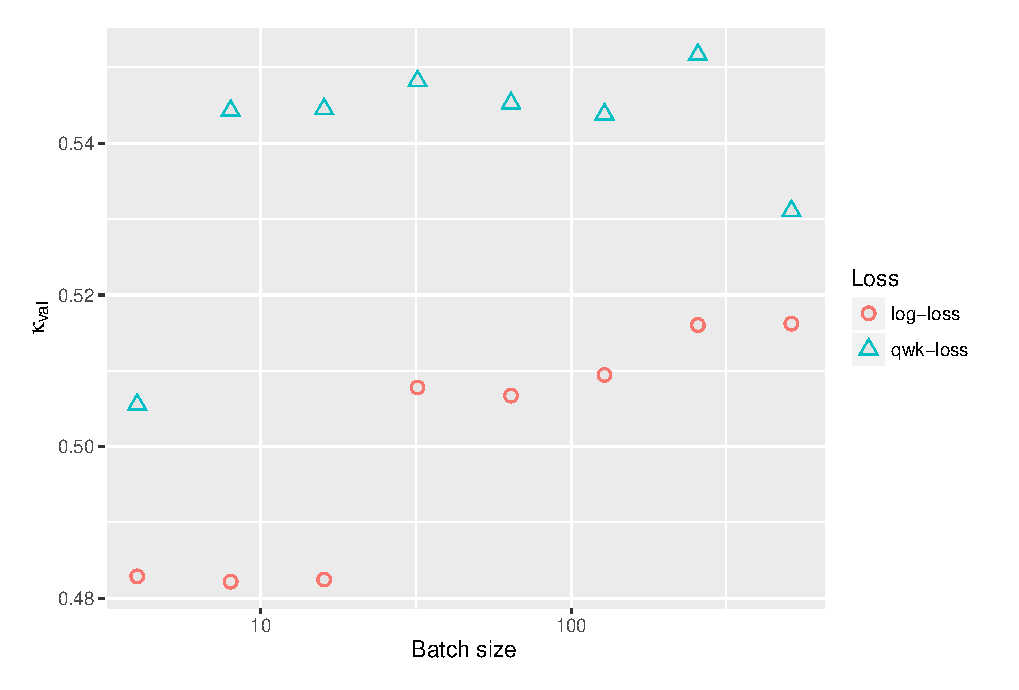
\includegraphics[width=0.5\textwidth]{./graphs/crowdflower-results.eps}
	\caption{$\kappa_{val}$ of the best model for every batch size  (case 1: search results relevance)}
	\label{fig:crowdflower}
\end{figure}

\begin{table}[h!]
	\centering
	\caption{List of all experiments for Case 1: Search results relevance}
	\label{tab:crowdflower}
	\resizebox{\columnwidth}{!}{ 
		\begin{tabular}{c|c|c|c|c|c|c}
			ID & BS & LR & $\kappa^{qwk\mbox{-}loss}_{val} 10^3$ & $Epoch^{qwk\mbox{-}loss}_{best}$ & $\kappa^{log\mbox{-}loss}_{val} 10^3$ & $Epoch^{log\mbox{-}loss}_{best}$\\
			\hline
			1 & \multirow{5}{*}{4}   & 1e-02 & 405 & 10 & 439 & 9\\
			2 &                      & 1e-03 & 485 & 6 & 476 & 6\\
			3 &                      & 5e-04 & \textbf{506} & 15 & \textbf{483} & 14\\
			4 &                      & 1e-04 & 503 & 19 & 467 & 3\\
			5 &                      & 1e-05 & 461 & 99 & 455 & 50\\
			\hline	
			6 & \multirow{5}{*}{8}   & 1e-02 & 450 & 13 & 444 & 6\\
			7 &                      & 1e-03 & \textbf{544} & 6 & \textbf{482} & 0\\
			8 &                      & 5e-04 & 524 & 9 & 475 & 18\\
			9 &                      & 1e-04 & 535 & 31 & 482 & 10\\
			10 &                     & 1e-05 & 445 & 99 & 479 & 50\\
			\hline	
			11 & \multirow{5}{*}{16} & 1e-02 & 504 & 18 & 425 & 3\\
			12 &                     & 1e-03 & 535 & 10 & 480 & 1\\
			13 &                     & 5e-04 & 543 & 11 & \textbf{480} & 1\\
			14 &                     & 1e-04 & \textbf{545} & 50 & 483 & 9\\
			15 &                     & 1e-05 & 395 & 99 & 479 & 86\\
			\hline	
			16 & \multirow{5}{*}{32} & 1e-02 & 515 & 12 & 436 & 2\\
			17 &                     & 1e-03 & 548 & 16 & 494 & 1\\
			18 &                     & 5e-04 & \textbf{548} & 17 & \textbf{508} & 4\\
			19 &                     & 1e-04 & 519 & 60 & 501 & 17\\
			20 &                     & 1e-05 & 385 & 99 & 485 & 99\\
			\hline	
			21 & \multirow{5}{*}{64} & 1e-02 & 520 & 10 & 473 & 8\\
			22 &                     & 1e-03 & 531 & 12 & 488 & 4\\
			23 &                     & 5e-04 & \textbf{545} & 37 & 506 & 9\\
			24 &                     & 1e-04 & 514 & 61 & \textbf{507} & 25\\
			25 &                     & 1e-05 & 377 & 99 & 400 & 99\\
			\hline	
			26 & \multirow{5}{*}{128} & 1e-02 & 513 & 4 & 479 & 5\\
			27 &                      & 1e-03 & \textbf{544} & 23 & 497 & 6\\
			28 &                      & 5e-04 & 527 & 31 & 499 & 8\\
			29 &                      & 1e-04 & 503 & 72 & \textbf{509} & 55\\
			30 &                      & 1e-05 & 317 & 99 &   0 & 0\\
			\hline	
			31 & \multirow{5}{*}{256} & 1e-02 & 510 & 8 & 490 & 1\\
			32 &                      & 1e-03 & \textbf{552} & 32 & \textbf{516} & 14\\
			33 &                      & 5e-04 & 490 & 21 & 507 & 24\\
			34 &                      & 1e-04 & 421 & 45 & 469 & 48\\
			35 &                      & 1e-05 & 189 & 99 & 61 & 34\\
			\hline	
			36 & \multirow{5}{*}{512} & 1e-02 & 512 & 18 & 488 & 7\\
			37 &                      & 1e-03 & \textbf{531} & 38 & \textbf{516} & 24\\
			38 &                      & 5e-04 & 509 & 64 & 493 & 27\\
			39 &                      & 1e-04 & 443 & 99 & 450 & 86\\
			40 &                      & 1e-05 & 15 & 4 & 41 & 43\\
			\hline			
		\end{tabular}
	}
\end{table}

After the study, we check the performance of the best model trained with qwk-loss and log-loss, using the test set (i.e. against never seen before records) consisting on 256,735 records. The test of the best model trained with qwk-loss reports a $\kappa_{test} = 0.500 \pm 0.043$ (95\% confidence). The best model trained with log-loss achieves a kappa in the test set of $\kappa_{test} = 0.468 \pm 0.050$ (95\% confidence). The difference between the two models is about a 6\% increase of the value of $\kappa_{test}$ (see fig. \ref{fig:retine-boxplot}).


\begin{figure}[!htb]
	\centering
	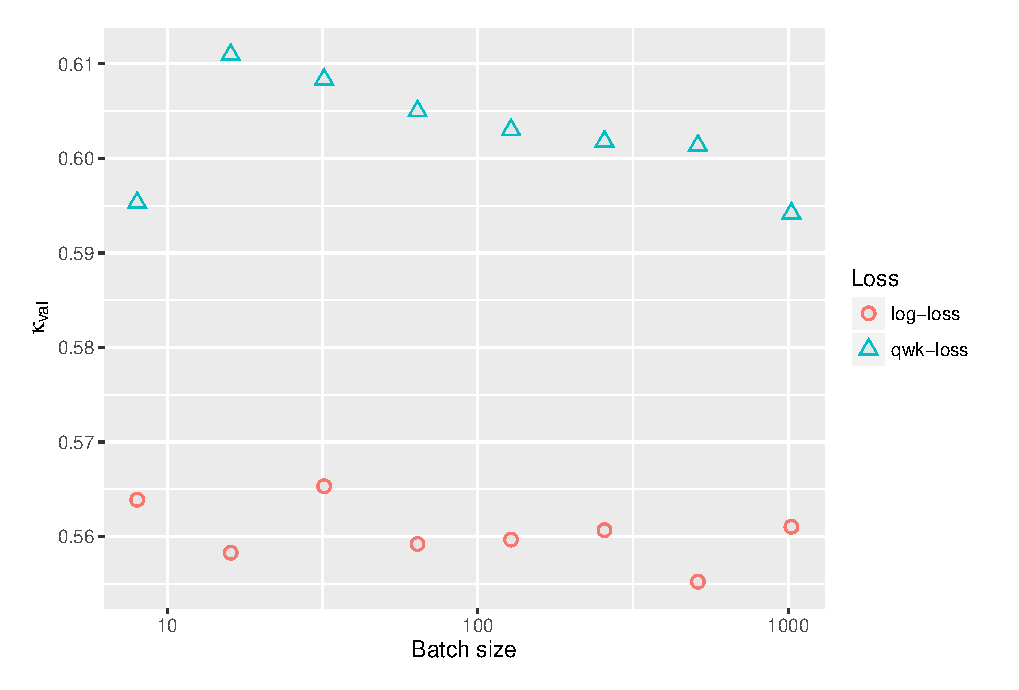
\includegraphics[width=0.5\textwidth]{./graphs/prudential-results.eps}
	\caption{$\kappa_{val}$ of the best model for every batch size (case 2: life insurance assessment)}
	\label{fig:prudential}
\end{figure}

\begin{table}[h!]
	\centering
	\caption{List of experiments for Case 2: Life insurance assessment}
	\label{tab:prudential}
	\resizebox{\columnwidth}{!}{ 
		\begin{tabular}{c|c|c|c|c|c|c}
			ID & BS & LR & $\kappa^{qwk\mbox{-}loss}_{val} 10^3$ & $Epoch^{qwk\mbox{-}loss}_{best}$ & $\kappa^{log\mbox{-}loss}_{val} 10^3$ & $Epoch^{log\mbox{-}loss}_{best}$\\
			\hline
			1 & \multirow{5}{*}{8}  & 1e-02 & 412 & 0 & 564 & 5\\
			2 &                     & 1e-03 & 593 & 3 & 550 & 4\\
			3 &                     & 5e-04 & 592 & 8 & 556 & 2\\
			4 &                     & 1e-04 & \textbf{595} & 11 & \textbf{560} & 4\\
			5 &                     & 1e-05 & 588 & 20 & 556 & 27\\
			\hline
			6 & \multirow{5}{*}{16} & 1e-02 & 570 & 1 & 555 & 8\\
			7 &                     & 1e-03 & 605 & 5 & 550 & 4\\
			8 &                     & 5e-04 & \textbf{611} & 7 & \textbf{558} & 2\\
			9 &                     & 1e-04 & 605 & 7 & 558 & 9\\
			10 &                    & 1e-05 & 596 & 14 & 554 & 28\\
			\hline
			11 & \multirow{5}{*}{32} & 1e-02 & 587 & 0 & 560 & 1\\
			12 &                     & 1e-03 & 604 & 2 & \textbf{565} & 3\\
			13 &                     & 5e-04 & \textbf{608} & 2 & 552 & 4\\
			14 &                     & 1e-04 & 603 & 11 & 562 & 11\\
			15 &                     & 1e-05 & 598 & 24 & 545 & 44\\
			\hline
			16 & \multirow{5}{*}{64} & 1e-02 & 587 & 0 & 547 & 7\\
			17 &                     & 1e-03 & \textbf{605} & 3 & 557 & 5\\
			18 &                     & 5e-04 & 603 & 4 & \textbf{559} & 4\\
			19 &                     & 1e-04 & 600 & 5 & 557 & 8\\
			20 &                     & 1e-05 & 595 & 38 & 542 & 30\\
			\hline
			21 & \multirow{5}{*}{128} & 1e-02 & 592 & 2 & 554 & 4\\
			22 &                      & 1e-03 & 602 & 5 & \textbf{560} & 2\\
			23 &                      & 5e-04 & \textbf{603} & 4 & 556 & 8\\
			24 &                      & 1e-04 & 599 & 7 & 558 & 18\\
			25 &                      & 1e-05 & 567 & 48 & 537 & 45\\
			\hline
			26 & \multirow{5}{*}{256} & 1e-02 & 589 & 6 & 555 & 1\\
			27 &                      & 1e-03 & \textbf{602} & 3 & 555 & 2\\
			28 &                      & 5e-04 & 598 & 6 & 555 & 1\\
			29 &                      & 1e-04 & 592 & 6 & \textbf{561} & 20\\
			30 &                      & 1e-05 & 589 & 49 & 515 & 26\\
			\hline
			31 & \multirow{5}{*}{512} & 1e-02 & \textbf{601} & 16 & \textbf{555} & 1\\
			32 &                      & 1e-03 & 601 & 5 & 548 & 5\\
			33 &                      & 5e-04 & 598 & 3 & 554 & 9\\
			34 &                      & 1e-04 & 598 & 15 & 548 & 19\\
			35 &                      & 1e-05 & 563 & 49 & 523 & 48\\
			\hline
			36 & \multirow{5}{*}{1024} & 1e-02 & 594 & 4 & 549 & 3\\
			37 &                       & 1e-03 & 592 & 5 & \textbf{561} & 7\\
			38 &                       & 5e-04 & \textbf{594} & 5 & 554 & 12\\
			39 &                       & 1e-04 & 593 & 21 & 547 & 22\\
			40 &                       & 1e-05 & 472 & 49 & 470 & 49\\
			\hline			
		\end{tabular}
	}
\end{table}


\subsection{Case 2. Life insurance assessment}

In figure \ref{fig:prudential}, the best results achieved on the training stage for every batch size and learning rate are shown. For each batch size, 5 LR values are tested. In bold we have the best $\kappa_{val}$ of each batch size. This are graphically displayed in fig. \ref{fig:prudential}.
Next, the best parameters are chosen for the two models and the performance is evaluated using the test set, consisting on 19,765 records. The test of the best model trained with qwk-loss reports a $\kappa_{test} = 0.618 \pm 0.016$ (95\% confidence). In the case of the best model trained with log-loss the value of kappa in the test set is $\kappa_{test} = 0.562 \pm 0.018$ (95\% confidence). A significant difference between the two best models in the test set is found, with about a 10\% increase of the value of $\kappa_{test}$ (see fig. \ref{fig:retine-boxplot}).


\subsection{Case 3. Diabetic retinopathy detection}

Table \ref{tab:qwk_cv} shows the collection of all the conducted experiments where \emph{input} represents the size of the input layer, \emph{BS} the batch size used in the experiment, \emph{LR} the learning rate, \emph{$\kappa_{train}$} the maximum value of $\kappa$ achieved during training over the training set, \emph{$\kappa_{val}$} the maximum value of $\kappa$ achieved during training over the validation set, \emph{gap} the difference between $\kappa_{train}$ and $\kappa_{val}$, \emph{epoch} the epoch where the maximum value of $\kappa_{val}$ is achieved and finally \emph{updates} the number of parameters updates required to achieve the maximum value of $\kappa_{val}$.


% Aquí taula 4
\begin{table}[h!]
	\centering
	\caption{List of experiments for Case 3: diabetic retinopathy detection}
	\label{tab:qwk_cv}
	\resizebox{\columnwidth}{!}{ 
	\begin{tabular}{c|c|c|c|c|c|c|c|c}
		Input & BS & Loss & LR	& $\kappa_{train} 10^3$ & $\kappa_{val} 10^3$ & Gap & Epoch & Updates $10^{-3}$\\	
		\hline
		\multirow{32}{*}{128} & \multirow{6}{*}{5} & \multirow{3}{*}{log} & $10^{-5}$ & 771 & 418 & 353 & 78 & 1560\\
		& & & $10^{-4}$ & 851 & \textbf{491} & 360 & 73 & 1460\\
		& & & $10^{-3}$ & 676 & 418 & 258 & 29 & 580\\\cline{3-9}
		& & \multirow{3}{*}{qwk} & $5 \times 10^{-5}$ & 545 & 402 & 143 & 50 & 1000\\
		& & & $10^{-5}$ & 646 & 439 & 207 & 70 & 1400\\
		& & & $10^{-4}$ & 497 & 326 & 171 & 31 & 620\\\cline{2-9}
		&\multirow{6}{*}{10} & \multirow{3}{*}{log} & $10^{-5}$ & 797 & 397 & 400 & 82 & 820\\
		& & & $10^{-4}$ & 874 & 455 & 419 & 81 & 810\\
		& & & $10^{-3}$ & 514 & 336 & 178 & 57 & 570\\\cline{3-9}
		& & \multirow{3}{*}{qwk} &  $10^{-5}$ & 774 & 476 & 298 & 82 & 820\\
		& & & $10^{-4}$ & 755 & 503 & 252 & 84 & 840\\
		& & & $10^{-3}$ & 596 & 289 & 307 & 95 & 950\\\cline{2-9}		
		& \multirow{6}{*}{15} & \multirow{3}{*}{log} & $10^{-5}$ & 803 & 368 & 435 & 79 & 527\\
		& & & $10^{-4}$ & 899 & 458 & 441 & 95 & 633\\
		& & & $10^{-3}$ & 868 & 447 & 421 & 80 & 533\\\cline{3-9}
		& & \multirow{3}{*}{qwk} & $5\times10^{-5}$ & 715 & 491 & 224 & 77 & 513\\
		& & & $10^{-4}$ & 800 & 526 & 274 & 77 & 513\\
		& & & $5\times10^{-4}$ & 823 & 523 & 300 & 72 & 480\\\cline{2-9}
		& \multirow{2}{*}{20} & log & $10^{-4}$ & 896 & 474 & 422 & 79 & 395\\\cline{3-9}
		& & qwk & $10^{-4}$ & 835 & \textbf{537} & 298 & 93 & 465\\\cline{2-9}
		& \multirow{6}{*}{25} & \multirow{3}{*}{log} & $10^{-5}$ & 821 & 315 & 506 & 96 & 384\\
		& & & $10^{-4}$ & 913 & 453 & 460 & 93 & 372\\
		& & & $10^{-3}$ & 849 & 382 & 467 & 70 & 280\\\cline{3-9}
		& & \multirow{3}{*}{qwk} & $10^{-5}$ & 808 & 423 & 385 & 95 & 380\\
		& & & $10^{-4}$ & 824 & 499 & 325 & 65 & 260\\
		& & & $10^{-3}$ & 655 & 447 & 208 & 80 & 320\\\cline{2-9}
		& \multirow{2}{*}{100} & \multirow{3}{*}{log} & $10^{-4}$ & 929 & 377 & 552 & 98 & 98\\
		& & & $10^{-3}$ & 947 & 444 & 503 & 99 & 99\\
		& & & $10^{-2}$ & 842 & 412 & 430 & 67 & 67\\\cline{3-9}
		& & \multirow{3}{*}{qwk} & $10^{-4}$ & 879 & 450 & 429 & 93 & 93\\
		& & & $10^{-3}$ & 798 & 455 & 343 & 71 & 713\\
		& & & $10^{-2}$ & - & - & - & - & -\\
		\hline	
		\multirow{10}{*}{256} & \multirow{2}{*}{5} & \multirow{1}{*}{log} & $10^{-4}$ & 871 & \textbf{571} & 300 & 52 & 1040\\\cline{3-9}
		& & \multirow{1}{*}{qwk} & $10^{-4}$ & 605 & 433 & 172 & 15 & 300\\\cline{2-9}
		&\multirow{2}{*}{10} & \multirow{1}{*}{log} & $10^{-4}$ & 903 & 566  & 337 & 75 & 750\\\cline{3-9}
		& & \multirow{1}{*}{qwk} & $10^{-4}$ & 832 & 616 & 216 & 70 & 700\\\cline{2-9}		
		& \multirow{2}{*}{15} & \multirow{1}{*}{log} & $10^{-4}$ & 925 & 556 & 369 & 98 & 653\\\cline{3-9}
		& & \multirow{1}{*}{qwk} & $10^{-4}$ & 878 & \textbf{622} & 256 & 93 & 620\\\cline{2-9}
		& \multirow{2}{*}{20} & \multirow{1}{*}{log} & $10^{-4}$ & 923 & 525 & 398 & 97 & 485\\\cline{3-9}
		& & \multirow{1}{*}{qwk} & $10^{-4}$ & 891 & 618 & 273 & 97 & 485 \\\cline{2-9}		
		& \multirow{2}{*}{30} & \multirow{1}{*}{log} & $10^{-4}$ & 925 & 514 & 411 & 93 & 310\\\cline{3-9}
		& & \multirow{1}{*}{qwk} & $10^{-4}$ & 900 & 586 & 314 & 98 & 327\\\cline{2-9}
		& \multirow{2}{*}{40} & \multirow{1}{*}{log} & $10^{-4}$ & 922 & 464 & 458 & 93 & 233\\\cline{3-9}
		& & \multirow{1}{*}{qwk} & $10^{-4}$ & 894 & 592 & 302 & 78 & 195\\\cline{2-9}
		\hline					
		\multirow{2}{*}{384} & \multirow{1}{*}{5} & \multirow{1}{*}{log} & $10^{-4}$ & 863 & \textbf{641} & 222 & 38 & 760\\\cline{2-9}
		& \multirow{1}{*}{15} & \multirow{1}{*}{qwk} & $10^{-4}$ & 889 & \textbf{698} & 191 & 93 & 620 \\\cline{2-9}
		\hline					
		\multirow{4}{*}{512} & \multirow{1}{*}{5} & \multirow{1}{*}{log} & $10^{-4}$ & 980 & \textbf{681} & 299 & 88 & 1760\\\cline{2-9}
		& \multirow{2}{*}{15} & \multirow{1}{*}{log} & $10^{-4}$ & 978 & 668 & 310 &  94 & 626\\\cline{3-9}
		&  & \multirow{1}{*}{qwk} & $10^{-4}$ & 884 & \textbf{717} & 167 & 86 & 573 \\\cline{2-9}
		& \multirow{1}{*}{20} & \multirow{1}{*}{qwk} & $10^{-4}$ & 903 & 701 & 202 & 89 & 445\\\cline{3-9}			
		\hline
	\end{tabular}
}
\end{table}

We can see that for every input size the maximum value achieved over the training set optimizing qwk-loss is always higher than the maximum value achieved optimizing log-loss (bold values). The gaps between both training and validation are also lower in the case of qwk-loss indicating a lower overfitting of the training data. We see that qwk-loss consistently reports better results than log-loss except for very low values of BS. In those cases, the qwk-loss performs worse than log-loss, but even in those cases the maximum value achieved by log-loss is lower than the best value of qwk-loss for the same model over the whole set of experiments.

In figure \ref{fig:best} we show a graphical representation of the maximum value of $\kappa_{val}$ for the different configurations. We can see that directly optimizing qwk-loss gives consistently better results than optimizing log-loss. Only in the case of very small batch sizes (for this application case, BS = 5) log-loss performs better than qwk-loss. This is probably due to the fact that qwk-loss uses a normalization term in the denominator that with not big enough batch sizes could cause instabilities in the gradient that affect the performance. In any case, even in those cases the results obtained with the log-loss are worse that the best achieved using the qwk-loss configuration.

\begin{figure}[!htb]
	\centering
	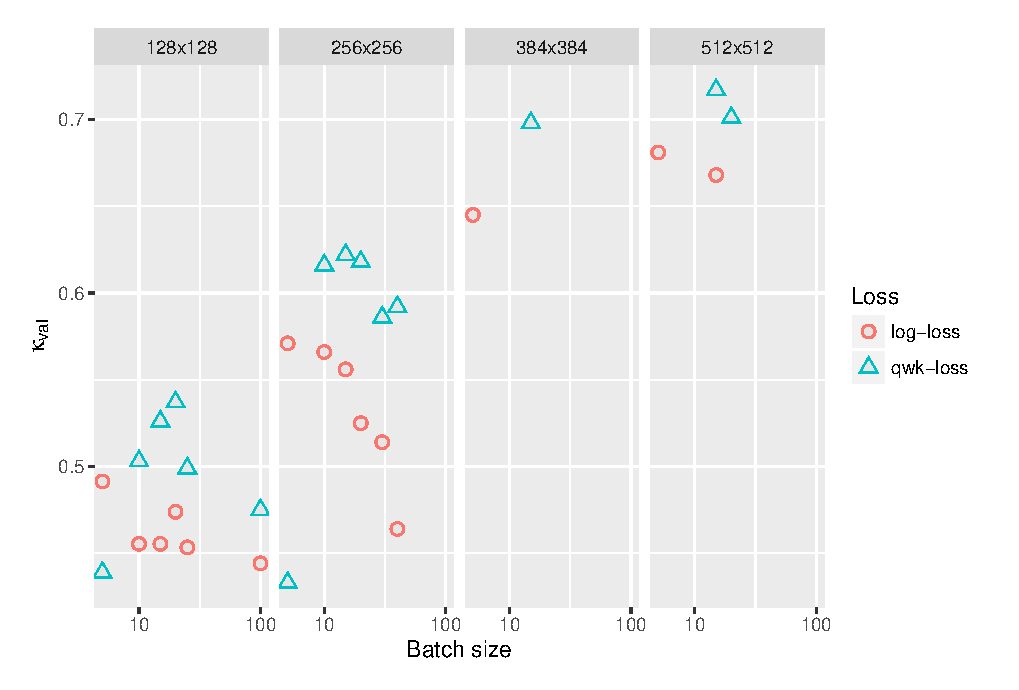
\includegraphics[width=0.5\textwidth]{./graphs/retine-results.eps}
	\caption{$\kappa_{val}$ achieved for the diabetic retinopathy detection use case in every experiment in function of the batch size and the loss function used}
	\label{fig:best}
\end{figure}

The optimal batch size for solving this diabetic retinopathy classification is of 5 in the case of using the log-loss and 15 in the case of the qwk-loss. For greater values of this hyper-parameter, the increase in precision of the calculation of the gradient does not report any advantage in the optimization. In the case of the log-loss a lower precision in the calculation of the gradient works better. It could probably be due to the fact that this imprecision in the calculation increases the stochasticity of the optimization and due to the fact that we are not optimizing directly the metrics index. This makes possible to explore adjacent zones that could work better for improving the metrics index than the ones that specifically improve the log-loss. Additionally, although smaller batch sizes give worse approximations of the gradient, the number of updates per epoch of the parameters of the model is greater. This seems to be an advantage in this case.

After all this study, we check the performance of the best model trained with qwk and log losses against the \emph{never seen before} 53,576 image test set. The test of the best model trained with qwk-loss reports a $\kappa_{test} = 0.740 \pm 0.006$ (95\% confidence). In the case of the same model trained with log-loss the value of $\kappa_{test} = 0.686 \pm 0.008$ (95\% confidence). The difference between the two best models in the test set is of more than a 7\% increase of the value of $\kappa$. (see case 3 in fig. \ref{fig:retine-boxplot})

Fig. \ref{fig:confusion-retine} helps to understand the difference between the performance of the optimized loss functions. This figure displays the histograms of the predicted classes for every true class. It can seen how the predicted histograms of the log-loss trained model are more scattered than the ones of the qwk-loss trained model. In those cases where there is a discrepancy between the real value and the predicted one, the model trained with the qwk-loss assign a category that are closer to the true category than the ones predicted by the log-loss trained model. This can be seen specially in the central category T2, where the distribution of qwk-loss model is concentrated in categories 1, 2 and 3 (with around 30\% each), while in the log-loss model, there are 25\% observations classified into class 0 as well as 10\% into class 4. This is of great importance when the classification is related with medical diagnosis. For a patient having severe retinopathy (class 4) it is better to be classified having a moderate or a proliferative one (closer classes) than to be classified as having a mild or as not having any retinopathy at all.

\begin{figure}[!htb]
	\centering
	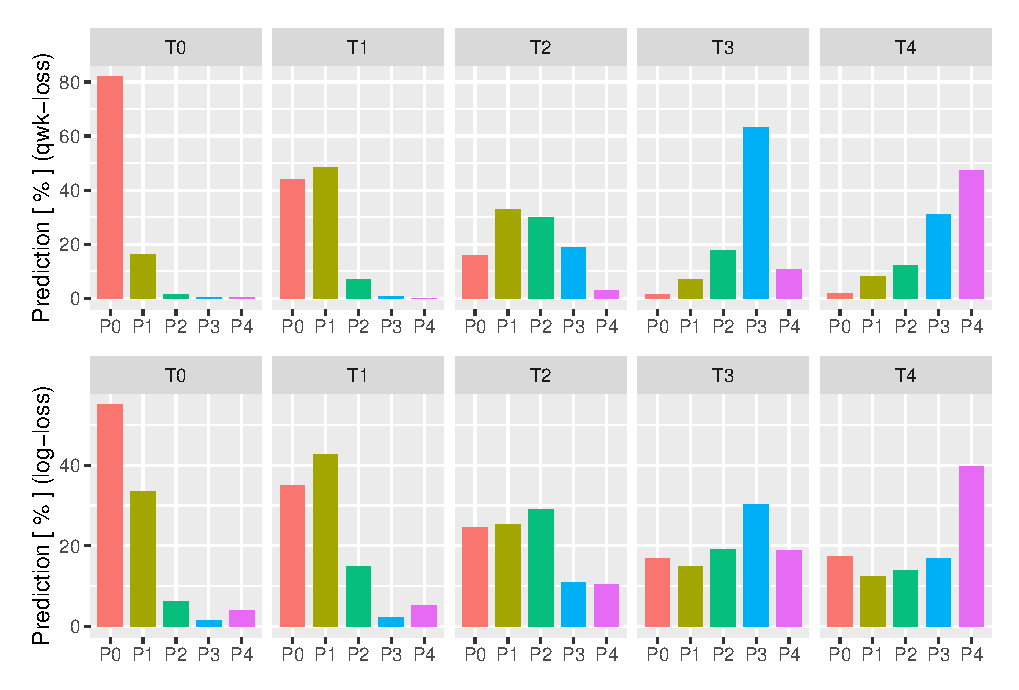
\includegraphics[width=0.5\textwidth]{./graphs/confusion-retine.eps}
	\caption{Histograms of the predicted classes for every real class over the test set for the best qwk-loss (above) and log-loss (below) trained models in the diabetic retinopathy multi-class classification use case}
	\label{fig:confusion-retine}
\end{figure}
 

\begin{table}[h!]
	\centering
	\caption{Summary of the difference in performance between qwk-loss and log-loss trained models in function of input size for the Diabetic retinopathy detection case}
	\label{tab:models}
	\resizebox{\columnwidth}{!}{ 
		\begin{tabular}{c|c|c|c|c|c|c|c}
			Input & \specialcell{Total\\Layers} & \specialcell[t]{Feature\\Layers} & \specialcell[t]{Classific.\\Layers} &  \specialcell[t]{Params\\$10^{-6}$} & $\kappa_{val}^{qwk\mbox{-}loss}$ & $\kappa_{val}^{log\mbox{-}loss}$ & $\Delta$\\
			\hline
			128x128 & 12 & 10 & 1 & 1.16 & 0.537 & 0.491 & 9.3 \%\\
			256x256 & 14 & 12 & 1 & 1.44 & 0.622 & 0.571 & 8.9 \%\\
			384x384 & 14 & 12 & 1 & 1.77 & 0.698 & 0.663 & 5.3 \%\\
			512x512 & 14 & 12 & 1 & 11.3 & 0.717 & 0.681 & 5.3 \%\\
			\hline
		\end{tabular}
}
\end{table}

\subsection{Overall discussion on the performance improvement}

In this section, the quality of the classification with the testing datasets is analyzed, although a brief comment has been made before on each case study.
Figure \ref{fig:retine-boxplot} shows the $\kappa$ index obtained on the testing data for the three case studies with the best model of every loss function. With this figure we can check if the difference between the two optimization techniques is statistically significant or not.
Improvement is clear for Case 2 and Case 3. Case 1 also has almost non-overlapping boxplots
but the $\kappa_{test}$ value achieved is more similar in the two models. However, in this case study the neural network used was the simplest one, thus the influence of the loss function in the final model is less. Improvement achieved with qwk-loss optimization is, thus, clear and supports the initial hypothesis of this research work.

\begin{figure}[!htb]
	\centering
	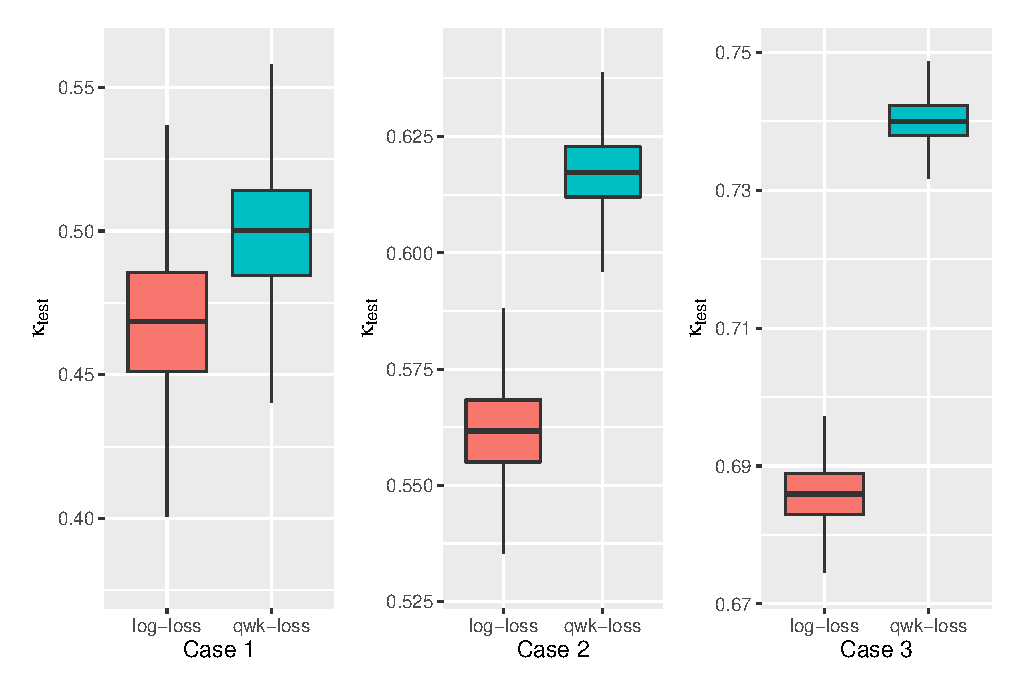
\includegraphics[width=0.4\textwidth]{./graphs/boxplots.eps}
	\caption{$\kappa_{test}$ confidence intervals for the log and qwk best models for the three studied cases}
	\label{fig:retine-boxplot}
\end{figure}

\section{Conclusions}

We presented a new loss function for training deep learning models in ordinal classification problems based on the optimization of the weighted kappa index. In contrast to the logarithmic loss that uses a uniform prior over the set of classes, this new loss function defines a penalization over the discrepancy that is proportional to a power of the distance (quadratically in the case of $\kappa$) that allows to encode the prior known information about the predefined ordering of the classes. 

We checked the performance of this new loss function with three different real-world case studies with diverse types of input data: textual in the first, categorical and numerical in the second and images in the third. Moreover, each case study was solved using decision models of increasing level of complexity: a linear classifier in the first, a multilayer perceptron in the second and a deep convolutional neural network in the third. 

The results presented in this paper show that with the direct optimization of the $\kappa$ index consistently better generalization results can be achieved than with the standard use of the logarithmic loss. Log-loss has to learn the predefined ordering of the classes from data and this seems to be a disadvantage. Results showed that, depending on the use case, between 6-10\% of improvement of $\kappa$ scores can be obtained from the direct optimization of the function.

This is a significant improvement that may be worth in many domains, such as the one of medical diagnosis, since an accurate detection of the level of severity of a disease usually has great influence on the treatment prescription and the possibility of minimizing bad consequences of the illness.

One minor drawback of the new loss is its low performance with very small batch sizes in the image classification study. The experiments show that for the retinopathy classification problem with batch sizes of 5, the performance of the function is lower than using the logarithmic loss. This parameter is for sure problem dependent and has to be taken into account as an important parameter to check in other image classification tasks that use a deep neural network.




\section*{Acknowledgments}
This work is supported by the URV grants 2014PFR-URV-B2-60 and 2015PFR-URV-B2-60, as well as, for the Spanish research projects PI15/01150 and PI12/01535 (Instituto de Salud Carlos III). The authors would like to thank to the Kaggle, Crowdflower, Prudential and EyePACS for providing the data used in this paper.


%\bibliographystyle{unsrt}
\bibliographystyle{model2-names}
\bibliography{retinopathy}

\end{document}

%%
